\documentclass{beamer}

\usepackage{lmodern}

\makeatletter
\newcommand\ChangeItemFont[3]{%
\renewcommand{\itemize}[1][]{%
  \beamer@ifempty{##1}{}{\def\beamer@defaultospec{#1}}%
  \ifnum \@itemdepth >2\relax\@toodeep\else
    \advance\@itemdepth\@ne
    \beamer@computepref\@itemdepth% sets \beameritemnestingprefix
    \usebeamerfont{itemize/enumerate \beameritemnestingprefix body}%
    \usebeamercolor[fg]{itemize/enumerate \beameritemnestingprefix body}%
    \usebeamertemplate{itemize/enumerate \beameritemnestingprefix body begin}%
    \list
      {\usebeamertemplate{itemize \beameritemnestingprefix item}}
      {\def\makelabel####1{%
          {%
            \hss\llap{{%
                \usebeamerfont*{itemize \beameritemnestingprefix item}%
                \usebeamercolor[fg]{itemize \beameritemnestingprefix item}####1}}%
          }%
        }%
  \ifnum\@itemdepth=1\relax
    #1%
  \else
  \ifnum\@itemdepth=2\relax
    #2%
  \else
  \ifnum\@itemdepth=3\relax
    #3%
  \fi%
  \fi%
  \fi%
  }
  \fi%
  \beamer@cramped%
  \raggedright%
  \beamer@firstlineitemizeunskip%
}}
\makeatother








\mode<presentation> {
  \usetheme{Warsaw}
  \setbeamercovered{transparent}
}

\usepackage[utf8]{inputenc}
\usepackage[spanish]{babel}
%\usepackage[latin1]{inputenc}

\usepackage{amsmath,amssymb}
\usepackage{graphicx}
\usepackage{fancyvrb}
\usepackage{color}
\usepackage{multirow}


\usepackage{soul}

\usepackage{tikz}
\usetikzlibrary{arrows,shapes}
\usetikzlibrary{shadows}
\usetikzlibrary{shapes.arrows}

\usepackage[3D]{movie15}

\newcommand\dq[1]{\textquotedblleft #1\textquotedblright}
\newcommand\sq[1]{\textquoteleft #1\textquoteright}

\title{Question answering de dominio abierto y de dominio cerrado}

\author{Julián Peller}

\date{Abril 2016} %

\subject{Defensa de tesis}

%\pgfdeclareimage[height=0.8cm]{university-logo}{logo}
%\logo{\includegraphics[width=8mm]{logo_uva.jpg}}



%\beamerdefaultoverlayspecification{<+->}


\AtBeginSubsection[]
{
   \begin{frame}<beamer>
   \frametitle{index.tex}
   \tableofcontents[currentsection,currentsubsection]
   \end{frame}
}

\AtBeginSection[]
{
   \begin{frame}<beamer>
   \frametitle{index.tex}
   \tableofcontents[currentsection]
   \end{frame}
}

\begin{document}

\begin{frame}
  \titlepage
\end{frame}

\begin{frame}
  \frametitle{index.tex}
  \tableofcontents[pausesections]
\end{frame}

% Introducción: qué es question answering, qué es esta tesis
\section{Introducción}

\subsection{Qué es question answering}

\begin{frame}
  \frametitle{¿Qué es question answering?}
  \begin{block}{Question Answering}<3->
      Es el proceso automatizado de generación de respuestas concretas para preguntas formuladas en lenguaje natural.
  \end{block}
  \bigskip

 \begin{alertblock}{Question}<2->
      ¿Quién desarrolló la teoría de la relatividad?
  \end{alertblock}

  \begin{columns}<3->
      \begin{column}{.5\textwidth}
      \end{column}
      \begin{column}{.1\textwidth}
      \begin{tikzpicture}[>=stealth, rotate border/.style={shape border uses incircle, shape border rotate=270}]
              \node[rotate border=-40, fill=black, minimum height=1.5cm, single arrow, single arrow head extend=.3cm, single arrow head indent=.1cm, inner sep=1.5pt] (arrow) {};
          \end{tikzpicture}
      \end{column}
      \begin{column}{.3\textwidth}
          %Question Answering
      \end{column}
      \begin{column}{.5\textwidth}

      \end{column}
  \end{columns}

  \begin{exampleblock}{Answer}<2->
      Albert Einstein.
  \end{exampleblock}
\end{frame}

\begin{frame}
\frametitle{Ejemplo IR}
\begin{figure}
  \centering
    \includegraphics[scale=.35]{graficos/i-r-example}
  \caption{Google como sistema de Information Retrieval}
  \label{fig:qa-example}
\end{figure}
\end{frame}


\begin{frame}
\frametitle{Ejemplo QA}
\begin{figure}
  \centering
    \includegraphics[scale=.5]{graficos/q-a-example}
  \caption{Google como sistema de Question Answering}
  \label{fig:qa-example}
\end{figure}
\end{frame}


\begin{frame}
  \frametitle{Clasificación}
  \begin{block}{Generalidad del dominio}<2->
    \begin{itemize}
      \item Dominio abierto o dominio cerrado
    \end{itemize}
  \end{block}
  \begin{block}{Tipo de datos}<3->
    \begin{itemize}
      \item Estructurados (Bases de datos)
      \item No estructurados (Colecciones de textos)
    \end{itemize}
  \end{block}
  \begin{block}{Soporte de preguntas}<4->
    \begin{itemize}
      \item Fácticas, listas, definiciones, modo, razón
      \item Cláusulas de tiempo, sin respuesta, etc.
    \end{itemize}
  \end{block}
\end{frame}


\subsection{Qué es esta tesis}

\begin{frame}
  \frametitle{Qué es esta tesis}
    \begin{block}{Brevemente}<2->
      Implementamos dos sistemas de question answering más o menos decentes.
    \end{block}
    \begin{exampleblock}{Dominio cerrado con soporte para inglés / Popescu World}<3->
      \begin{itemize}
          \item Base de datos relacional de juguete
          \item Modelo teórico de \textit{tratabilidad semántica}
          \item Traduce preguntas a consultas SQL
      \end{itemize}
    \end{exampleblock}
    \begin{alertblock}{Dominio abierto con soporte multilingüe / Multilingual Qanus}<4->
      \begin{itemize}
          \item Wikipedia(s) como base de conocimientos
          \item Framework Qanus y librería Freeling
          \item Basado en IR + NLP + heurísticas
      \end{itemize}
    \end{alertblock}
\end{frame}

\section{Dominio cerrado (Popescu/World)}
\subsection{Introducción}

\begin{frame}
  \frametitle{Introducción}\fontsize{8.0pt}{8.0}\selectfont
  \begin{block}{Modelo teórico: tratabilidad semántica (Popescu et al.)}
    \begin{itemize}
          \item QADB: Question answering como interfaz para una base de datos
          \item \textbf{Tratabilidad semántica de una pregunta $q$ en el contexto de una DB $d$}.
          \item Funcionalidad acotada y soporte solo para el inglés.
    \end{itemize}
  \end{block}

  \begin{block}{Pregunta}<2->
      \textbf{When was Albert Einstein born?}
  \end{block}
  \begin{columns}<3->
      \begin{column}{.5\textwidth}
      \end{column}
      \begin{column}{.1\textwidth}
      \begin{tikzpicture}[>=stealth, rotate border/.style={shape border uses incircle, shape border rotate=270}]
              \node[rotate border=-40, fill=black, minimum height=.4cm, single arrow, single arrow head extend=.2cm, single arrow head indent=.1cm, inner sep=1.5pt] (arrow) {};
          \end{tikzpicture}
      \end{column}
      \begin{column}{.3\textwidth}
          %Question Answering
      \end{column}
      \begin{column}{.5\textwidth}

      \end{column}
  \end{columns}

  \begin{exampleblock}{Consulta SQL}<3->
\textbf{{\color{purple}SELECT} birth\_date \newline
      {\color{purple}FROM} scientists\newline
      {\color{purple}WHERE} name $=$ {\color{green}`Albert Einstein'}
      }
  \end{exampleblock}
  \begin{columns}<4->
      \begin{column}{.5\textwidth}
      \end{column}
      \begin{column}{.1\textwidth}
      \begin{tikzpicture}[>=stealth, rotate border/.style={shape border uses incircle, shape border rotate=270}]
              \node[rotate border=-40, fill=black, minimum height=.4cm, single arrow, single arrow head extend=.2cm, single arrow head indent=.1cm, inner sep=1.5pt] (arrow) {};
          \end{tikzpicture}
      \end{column}
      \begin{column}{.3\textwidth}
          %Question Answering
      \end{column}
      \begin{column}{.5\textwidth}

      \end{column}
  \end{columns}

  \begin{alertblock}{Respuesta}<4->
      \textbf{March 14th, 1879}
  \end{alertblock}

\end{frame}



\subsubsection*{Base de datos}\fontsize{9.5pt}{8.2}\selectfont
\begin{frame}
\frametitle{Base de datos: World (Country, City y CountryLanguage)}
\begin{figure}
    \includegraphics[width=9.823cm,height=6.004cm]{graficos/fuentes/world-db.png}
\end{figure}
\end{frame}



\subsection{Modelo teórico}


\begin{frame}[<+->]
  \frametitle{Tratabilidad semántica / motivación}
      \begin{itemize}
          \item La complejidad de las preguntas en lenguaje natural es arbitraria.
          \item Distinguir un subconjunto 1) \textit{tratable} (simple) y 2) \textit{abarcativo}
          \begin{itemize}
            \item La {\color{blue}\textbf{tratabilidad semántica}} formaliza esta clase
          \end{itemize}
          \item Rechazar y pedir reformulación de las no tratables
          \begin{itemize}
            \item Es mejor no dar respuesta a dar una mala. 
            \item Conservar la confianza en el sistema.
          \end{itemize}
      \end{itemize}

    \begin{alertblock}{Tratable}
     La tratabilidad está dada por cualidades estructurales pero también por el contenido
      \begin{itemize}
          \item atributo $=$ valor (forma de gobierno = monarquía)
          \item valor suelto - atributo implícito 
      \end{itemize}

    \end{alertblock}
\end{frame}

\begin{frame}[<+->]
  \frametitle{Tratabilidad semántica / ejemplos}

    \begin{block}{Ejemplos}
      \begin{enumerate}
          \item ¿Qué países asiáticos son monarquías? $\rightarrow$ {\color{green}Sí}
          \item ¿Qué países de Asia no desarrollaron formas de gobierno basadas en las ideas de la Ilustración? $\rightarrow$ {\color{red}No}
          %\item ¿Qué países del continente de Lenin son monarquías? $\rightarrow$ {\color{red}No}
          %\item ¿Qué países asiáticos tienen como gobierno una monarquía? $\rightarrow$ {\color{green}Sí}
          \item ¿Qué países del continente asiático tienen como forma de gobierno una monarquía? $\rightarrow$ {\color{green}Sí}
          \item ¿Qué países del continente que está al este de Europa y contiene a Rusia tiene esa forma de gobierno en la que manda una sola persona? $\rightarrow$ {\color{red}No}
          \item ¿Quiénes son los líderes de las monarquías asiáticas? $\rightarrow$ {\color{green}Sí}
      \end{enumerate}
    \end{block}
\end{frame}

%\fontsize{7.0pt}{6.0}\selectfont
\begin{frame}[<+->]
  \frametitle{Tratabilidad semántica / intuición}
    \begin{block}{Una pregunta semánticamente tratable tiene:}
      \begin{itemize}
          \item {\color{blue}Atributos} y {\color{blue}Valores} apareados
           \begin{itemize}
             \item  ¿Qué países tienen como {\color{blue}forma} de {\color{blue}gobierno} una {\color{blue}monarquía}?
           \end{itemize}
          \item {\color{red}Valores} sueltos (atributo implícito)
           \begin{itemize}
             \item ¿Qué países son {\color{red}monarquías}?
           \end{itemize}
          \item Una {\color{green}Q-word} (Qué, quién, cuándo) apareada con un atributo o suelta (atributo implícito)
          \begin{itemize}
            \item ¿{\color{green}Quiénes} son los {\color{green}líderes} de las monarquías asiáticas?
            \item ¿{\color{green}Qué} países son monarquías?
          \end{itemize}
          \item Marcadores sintácticos
          \item Menciones sueltas a {\color{orange}relaciones}
      \end{itemize}
    \end{block}
\end{frame}



%\fontsize{7.0pt}{6.0}\selectfont
\begin{frame}[<+->]
  \frametitle{Tratabilidad semántica / intuición}
    \begin{exampleblock}{Abarcativo e intuitivamente traducible a una consulta SQL}
      \begin{itemize}
          \item ¿{\color{green}Qué} {\color{orange}países} del {\color{blue}continente} {\color{blue}asiático} tienen como {\color{blue}forma} de {\color{blue}gobierno} una {\color{blue}monarquía}?
            \begin{itemize}
              \item Debería ser algo como: {\color{purple}SELECT} Country.Name {\color{purple}FROM} Country {\color{purple}WHERE} Continent=\textbf{Asia} {\color{purple}AND} GovernmentForm=\textbf{Monarchy}
            \end{itemize}
            \item ¿{\color{green}Qué} {\color{orange}países} {\color{red}asiáticos} son {\color{red}monarquías}?
            \begin{itemize}
              \item Misma query, pero los atributos implícitos y deben \dq{descubrirse}
            \end{itemize}
            \item ¿{\color{green}Quiénes} son los {\color{green}líderes} de las {\color{red}monarquías} {\color{red}asiáticas}?
            \begin{itemize}
              \item Q-word apareada explicitamente con atributo: {\color{purple}SELECT} Country.HeadOfState {\color{purple}FROM} Country {\color{purple}WHERE} Continent=\textbf{Asia} {\color{purple}AND} GovernmentForm=\textbf{Monarchy}
            \end{itemize}
      \end{itemize}
    \end{exampleblock}
    
\end{frame}

\subsection{Implementación}


\begin{frame}[<+->]\fontsize{7.5pt}{7.2}\selectfont
  \frametitle{Módulos principales}
  \begin{block}{Lexicón: dominio semántico}
    \begin{itemize}
      \item Elementos de la DB $\rightarrow$ Wordnet $\rightarrow$ Lexicón (sinónimos)
      \item Todas las palabras que el sistema entiende están en el lexicón (tokens)
      \item Salto de las palabras a los elementos de la DB
      \begin{itemize}
        \item  \tiny{region, part, area, neighborhood, realm  $\rightarrow$ Atributo Country.Region  }
        \item  \tiny{city, metropolis, urban center  $\rightarrow$ Relación (tabla) City}
      \end{itemize}
    \end{itemize}
  \end{block}
  \begin{alertblock}{Tokenizer: pregunta $\rightarrow$ tokens del lexicón}
      \begin{itemize}
          \item Pregunta $q$ $\rightarrow$ Marcadores sintácticos (se tiran) + términos del lexicón
          \item Si no se puede, la pregunta ya no es tratable
          \item Propone particiones de $q$ en items del lexicón (tokenizaciones completas)
      \end{itemize}
  \end{alertblock}
  \begin{exampleblock}{Matcher: (tokens $\rightarrow$ elementos) + apareo + desambiguación}
      \begin{itemize}
          \item Filtra tokenizaciones válidas (\dq{traducciones}) con max flow (grafos)
          \item Descubre atributos implícitos
          \item Genera pares de atributos y valores y un atributo con la qword
          \item Desambigua sobreyecciones token $\rightarrow$ elemento al maximizar el flujo
    \end{itemize} 
  \end{exampleblock}
\end{frame}


% \begin{frame}[<+->]
%   \frametitle{Modulos principales}
%   \begin{block}{Lexicón: dominio semántico}
%     \begin{itemize}
%       \item Elementos de la DB $\rightarrow$ Wordnet $\rightarrow$ Lexicón (sinónimos)
%       \item \textbf{Elementos} de una DB: Relaciones, Atributos y Valores
%       \item Cada item del lexicón se llama \textbf{token}
%       \item Cada token es un sinónimo para uno o más elementos de la base de datos (\textbf{\dq{se corresponde con}})
%       \begin{itemize}
%             \item Esta relación va a ser el \dq{salto} entre las palabras y los elementos de la DB
%           \end{itemize}
%       \item Una pregunta \textit{tratable} va a constar de \textit{tokens} + marcadores sintácticos
%       %\item \fontsize{7.5pt}{7.2}\selectfont Notas: TokenAugmenter. Polisemia. Problemas.
%     \end{itemize}
%   \end{block}
%   \begin{alertblock}{Tokenizer}
%       \begin{itemize}
%           \item Elimina marcadores sintácticos
%           \item Rompe la pregunta y consulta al lexicón (¿a qué tokens pertenece esta palabra?)
%           \item Genera todas las particiones posibles de la pregunta en tokens del lexicón 
%           \begin{itemize}
%             \item Cada partición en tokens se llama \textit{tokenización completa}
%           \end{itemize}
%       \end{itemize}
%     \end{alertblock}
    
%     \begin{exampleblock}{Matcher}<1->
%       \begin{itemize}
%           \item Elimina marcadores sintácticos
%           \item Rompe la pregunta y consulta al lexicón (¿a qué tokens pertenece esta palabra?)
%           \item Genera todas las particiones posibles de la pregunta en tokens del lexicón 
%           \begin{itemize}
%             \item Cada partición en tokens se llama \textit{tokenización completa}
%           \end{itemize}
%       \end{itemize}
%     \end{exampleblock}
% \end{frame}


% \fontsize{9.5pt}{7.2}\selectfont
% \begin{frame}[<+->]
%   \frametitle{qword, compatibilidad}
%    \begin{itemize}
      
%       \item \textbf{Qwords} - pronombres interrogativos
%       \begin{itemize}
%         \item \{What, where, which, when, who\}, \{Qué, dónde, cuál, cuándo, quién\}
%         \item Funcionan como valores especiales (el valor preguntado)
%       \end{itemize}
%       \item \textbf{Compatibilidad}
%       \begin{itemize}
%           \item Valor $\rightarrow$ Atributo (Macri $\rightarrow$ HeadOfState)
%           \item Atributo  $\rightarrow$  Relación (HeadOfState $\rightarrow$ Country)
%           \item Valor $\rightarrow$ Relaciones de sus atributos (Macri $\rightarrow$ Country)
%           \item {\color{blue}Q-words $\rightarrow$ Atributos} (A manos)
%           \begin{itemize}
%             \item Who $\rightarrow$ HeadOfState, When $\rightarrow$ IndependenceYear , What $\rightarrow$ Varios atributos.
%           \end{itemize}
%       \end{itemize}
%     \end{itemize}
% \end{frame}


% \begin{frame}[<+->]
% \frametitle{Tokenización completa}

% \begin{block}{\textbf{Tokenización completa de una pregunta \textit{q}}}
%   \begin{itemize}
%     \item Una partición de tokens de la pregunta $q$
%     \item Pregunta tratable $\Leftrightarrow$ Marcadores sintácticos + tokens del lexicón
%    \end{itemize}
% \end{block}


% \end{frame}


% \fontsize{11pt}{7.2}\selectfont
% \begin{frame}
% \frametitle{Ejemplo}
% \begin{figure}
%   \centering
%     \includegraphics[scale=.7]{graficos/popescu-example}
%   \caption{La traducción de la pregunta ``What are the HP jobs on a Unix system?'' a una consulta SQL}
%   \label{fig:popescu-example}
% \end{figure}
% \end{frame}

% \begin{frame}[<+->]
% \frametitle{Matcher}
   
%    \begin{block}{Matcher}
%      \begin{itemize}
%       \item Input
%       \begin{itemize}
%         \item El tokenizer generó una más particiones de $q$ en items del lexicón (tokenizaciones)
%         \item Cada item mapea a uno o más elementos de la DB.
%       \end{itemize}
%       \item El matcher filtra mapeos válidos (\dq{traducciones válidas})
%         \begin{itemize}
%           \item  Relaciona cada \textbf{valor} con un único \textbf{atributo}, implícito o explícito usando un algoritmo de max flow.
%            \item Cada {\color{blue}atributo} del mapeo tiene un {\color{blue}valor} o {\color{green}qword} compatible y sintácticamente asociado.
%         \end{itemize}
%     \end{itemize} 
%   \end{block}
  
%   \begin{itemize}
%     \item Las aristas implicadas en el flujo máximo asocian 
%     \begin{enumerate}
%       \item los tokens de valor y de atributo y los correspondientes elementos (valores y atributos, respectivamente) de la DB y 
%       \item pares de valores y atributos entre sí.
%     \end{enumerate}
%     \end{itemize}
          
% \end{frame}

% \subsection{Implementación}

% \begin{frame}
%   \frametitle{Ejemplo}

%   \begin{figure}
%     \centering
%       \includegraphics[scale=0.3]{graficos/popescu-example-2}
%     \caption{El grafo de atributos y valores del Matcher para la pregunta ``What are the HP jobs on a Unix system?''}
%     \label{fig:popescu-example-2}
%   \end{figure}

% \end{frame}

\begin{frame}[<+->] \fontsize{9.5pt}{8.2}\selectfont
  \frametitle{Traducción válida / Query}    
    \begin{exampleblock}{Traducción válida}
     Cada máximo flujo genera pares atributo-valor y un par atributo-qword. Si sus tokens de atributo y de valor explícitos están sintácticamente asociados, entonces decimos que es una \textbf{traducción válida} de $q$
    \end{exampleblock}

  \begin{alertblock}{Semánticamente tratable}
    Una pregunta es \textbf{semánticamente tratable} si tiene una q-word y al menos una traducción válida
  \end{alertblock}

    \begin{block}{Una traducción válida de $q$ se traduce trivialmente a una consulta SQL}        
    \begin{tabular}{ r | l }
    {\color{purple}SELECT} &  Atributo apareado con la qword \\
    {\color{purple}WHERE} & Pares de atributos y valores apareados (implícitos y explícitos)\\
    {\color{purple}FROM} & Todas las relaciones mencionadas \\
    \end{tabular}
    \end{block}


    %\footnotetext[1]{\tiny{Falta una condición sobre tokens de relación que no es esencial mencionar}}

\end{frame}

% \fontsize{9.5pt}{8.2}\selectfont
% \begin{frame}
% \frametitle{Asociación sintáctica / Charniak parse tree}
% \Tree [.S1 [.WHNP [.WP What ] ] [.SQ [.VP [.AUX are ] [.{\color{red}NP} [.DT the ] [.{\color{red}NNP} {\color{red}HP} ] [.{\color{red}NNS} {\color{red}jobs} ] ] [.PP [.IN on ] [.{\color{red}NP} [.DT a ] [.{\color{red}NNP} {\color{red}Unix} ] [.{\color{red}NN} {\color{red}system} ] ] ] ] ] [.. ? ] ] \\
% {\color{red}Regla 1 - Sustantivos \dq{hermanos}}

% \end{frame}

% \begin{frame}
% \frametitle{Asociación sintáctica / Charniak parse tree}
% \Tree [.{\color{blue}S1} [.{\color{blue}WHNP} [.{\color{blue}WP} {\color{blue}What} ] ] [.{\color{blue}SQ} [.{\color{blue}VP} [.AUX are ] [.{\color{blue}NP} [.DT the ] [.{\color{blue}NNP} {\color{blue}HP} ] [.{\color{blue}NNS} {\color{blue}jobs} ] ] [.PP [.IN on ] [.NP [.DT a ] [.NNP Unix ] [.NN system ] ] ] ] ] [.. ? ] ] \\
% {\color{blue}Regla 2: qwords a sustantivos}

% \end{frame}


\subsubsection*{Ejemplos}

\begin{frame}[t]
\frametitle{Ejemplo 1: ``Who is the head of state of Zimbabwe?''}
Ejemplo 1:\newline
  \Large{``Who is the head of state of Zimbabwe?''}
\end{frame}

\begin{frame}[t]
\frametitle{Ejemplo 1: Tokenizer}
1. Separar, sacar puntuaciones, pasar a lower case, tirar stopwords:\newline
  \Large{\{{\color{blue}w}ho, {\color{red}\st{is}}, {\color{red}\st{the}}, head, {\color{red}\st{of}}, state, {\color{red}\st{of}}, {\color{blue}z}imbabwe\}}
\end{frame}


\begin{frame}[t]
\frametitle{Ejemplo 1: Tokenizer}
1. Separar, sacar puntuaciones, pasar a lower case, tirar stopwords:\newline
  \Large{\{who, head, state, zimbabwe\}}
\end{frame}

\begin{frame}[t]
\frametitle{Ejemplo 1: Tokenizer - tokens para who}
2. Obtener tokens para cada lema \tiny{(items del lexicón, sinónimo de 1+ elementos de la DB)} \newline
    \Large{$getTokens(who)\ \rightarrow \{$'who'$\}$}
\end{frame}

\begin{frame}[t]
\frametitle{Ejemplo 1: Tokenizer - tokens para head}
2. Obtener tokens para cada lema \newline
    \Large{$
    getTokens(head)\ \rightarrow \{$ 'head country', 'head teacher body politic', 'head body politic', 'head teacher land', 'read / write head dos', 'heading provincial', 'heading state', 'heading commonwealth', 'read / write head body politic', 'head word land', 'head state of matter', 'read / write head provincial', 'read / write head state department', 'head province',  'heading res publica', 'read / write head nation', (51 más)...$\}$}
\end{frame}

\begin{frame}[t]
\frametitle{Ejemplo 1: Tokenizer - tokens para state}
2. Obtener tokens para cada lema \newline
  \Large{ $getTokens(state)\ \rightarrow  \{$'heart eastern united states', 'centre eastern united states', 'central eastern united states', 'centrical eastern united states', 'midsection eastern united states', 'midriff eastern united states', 'centric eastern united states', 'center eastern united states', 'north western united states', (702 más)...$\}$}
\end{frame}

\begin{frame}[t]
\frametitle{Ejemplo 1: Tokenizer - tokens para Zimbabwe}
2. Obtener tokens para cada lema \newline
  \Large{$getTokens(zimbabwe)\ \rightarrow \{$'zimbabwe', 'republic of zimbabwe', 'capital of zimbabwe'$\}$}

\end{frame}

\begin{frame}[t]
\frametitle{Ejemplo 1: Tokenizer - intersección}
3. Filtrar solo tokens cuyos lemas estén en la pregunta\newline
  \Large{$getTokens(zimbabwe)\ \rightarrow \{$'zimbabwe', {\color{red}\st{'republic of zimbabwe'}}, {\color{red}\st{'capital of zimbabwe'}}$\}$ }
\end{frame}


\begin{frame}[t]
\frametitle{Ejemplo 1: Tokenizer - intersección}
3. Filtrar solo tokens cuyos lemas estén en la pregunta\newline
  \Large{
    $getTokens(zimbabwe) \rightarrow \{$'zimbabwe'$\}$\newline
    $getTokens(who)\ \rightarrow \{$'who'$\}$\newline
    $getTokens(head) \rightarrow \{$'head state'$\}$\newline
    $getTokens(state) \rightarrow  \{$'state','head state'$\}$
}
\end{frame}

\begin{frame}[t]
\frametitle{Ejemplo 1: ``Who is the head of state of Zimbabwe?''}
 5. Generar el conjunto de partes de todos contra todos (\textit{tokenizaciones}).\newline
  \Large{
      \{'state', 'zimbabwe'\},\newline
      \{ 'who', '{\color{red}state}', 'head {\color{red}state}', 'zimbabwe'\},\newline
      \{ 'who', 'head state', 'zimbabwe'\},\newline
      ...
  }\newline

\normalsize{
\begin{block}{Tokenización completa}  
  Quedarse solo con los que:
  \begin{itemize}
    \item Cubren la palabras no stopwords de la pregunta
    \item No tienen palabras {\color{red}repetidas}
  \end{itemize}
  
\end{block}
}
\end{frame}

\begin{frame}
\frametitle{Ejemplo 1: Tokenizaciones completas}

\begin{center}

$q = \text{``Who is the head of state of Zimbabwe?''}$
\end{center}
 \begin{equation*}
    CompleteTokenizations(q) = \begin{cases}
               \{\text{who, head state, zimbabwe}\}\} \\
           \end{cases}
\end{equation*}

\end{frame}

\begin{frame}[t]
\frametitle{Ejemplo 1: Lexicón - Tokens $\rightarrow$ Elementos}
Obtener elementos de la DB para cada token\newline
  \Large{
    $who \rightarrow Who$ (Qword compatible con HeadOfState) \newline
    $\text{head state} \rightarrow HeadOfState$ (Atributo de Country) \newline
    $zimbabwe \rightarrow Zimbabwe$ (Valor de Country.Name)\newline
    }
\end{frame}

\begin{frame}
\frametitle{Ejemplo 1: Matcher - Grafo de atributos y valores}
\begin{figure}
  \centering
    \includegraphics[scale=.33]{graficos/presentacion/ejemplo-grafo-matcher-1-2}
    \caption{1. Nodos Fuente (S) y Sumidero (T)}
\end{figure}

\end{frame}

\begin{frame}
\frametitle{Ejemplo 1: Matcher - Grafo de atributos y valores}
\begin{figure}
  \centering
    \includegraphics[scale=.33]{graficos/presentacion/ejemplo-grafo-matcher-1-3}
    \caption{2. Tokens de valor (palabras), desde S, con $f=1$}
\end{figure}
\end{frame}

\begin{frame}
\frametitle{Ejemplo 1: Matcher - Grafo de atributos y valores}
\begin{figure}
  \centering
    \includegraphics[scale=.33]{graficos/presentacion/ejemplo-grafo-matcher-1-4}
    \caption{3. Valores (DB) asociados a los tokens, con $f=1$}
\end{figure}
\end{frame}

\begin{frame}
\frametitle{Ejemplo 1: Matcher - Grafo de atributos y valores}
\begin{figure}
  \centering
    \includegraphics[scale=.33]{graficos/presentacion/ejemplo-grafo-matcher-1-5}
    \caption{4. Atributos (DB) asociados a los Valores, con $f=1$}
\end{figure}
\end{frame}

\begin{frame}
\frametitle{Ejemplo 1: Matcher - Grafo de atributos y valores}
\begin{figure}
  \centering
    \includegraphics[scale=.33]{graficos/presentacion/ejemplo-grafo-matcher-1-5-2}
    \caption{5. Repite Atributos, para forzar $f=1$ por Atributo}
\end{figure}
\end{frame}

\begin{frame}
\frametitle{Ejemplo 1: Matcher - Grafo de atributos y valores}
\begin{figure}
  \centering
    \includegraphics[scale=.33]{graficos/presentacion/ejemplo-grafo-matcher-1-5-3}
    \caption{6. Tokens de atributo, linkeados a Atributos con $f=1$}
\end{figure}
\end{frame}

\begin{frame}
\frametitle{Ejemplo 1: Matcher - Grafo de atributos y valores}
\begin{figure}
  \centering
    \includegraphics[scale=.33]{graficos/presentacion/ejemplo-grafo-matcher-1-6}
    \caption{6. Nodos I y E, con $f=tokens_{attr}$ y $f=tokens_{val} - tokens_{attr}$}
\end{figure}
\end{frame}


\begin{frame}[t]
\frametitle{Ejemplo 1: Matcher - notas}
\Large{``{\color{blue}Who} \st{is} \st{the} {\color{blue}head} \st{of} {\color{blue}state} \st{of} {\color{red}Zimbabwe}?''}
\normalsize{
\begin{itemize}
  \item {\color{blue}head state} es el Atributo {\color{blue}Country.HeadOfState}
  \item {\color{blue}Who} es un Valor y está apareado con {\color{blue}Country.HeadOfState} 
  \item {\color{red}Zimbabwe} es un Valor y está apareado con {\color{red}Country.Name} (implícito)
  \item No desambigua nada (los tokens tiene un solo elemento asociado)
\end{itemize}
}
\bigskip
Se chequea que los tokens de atributo y de valor explícitos apareados (`who' y `head state') estén sintácticamente asociados

\end{frame}

% \begin{frame}[t]
% \frametitle{Ejemplo 1: Matcher - Asociación sintáctica - Regla 1}
% \Large{Regla 1: who $\rightarrow$ head}
% \begin{center}
% \begin{figure}
%   \centering
%     \includegraphics[scale=.5]{graficos/presentacion/ejemplo-charniak-2}
% \end{figure}

% \end{center}
% \end{frame}

% \begin{frame}[t]
% \frametitle{Ejemplo 1: Matcher - Asociación sintáctica - Regla 6}
% \Large{Regla 6: head $\rightarrow$ state}
% \begin{center}

% \begin{figure}
%   \centering
%     \includegraphics[scale=.5]{graficos/presentacion/ejemplo-charniak-1}
% \end{figure}
% \end{center}
% \end{frame}

% \begin{frame}[t]
% \frametitle{Ejemplo 1: Generador de Queries}
% \Large{{\color{blue}Who} \st{is} \st{the} {\color{blue}head} \st{of} {\color{blue}state} \st{of} {\color{red}Zimbabwe}? 
% \bigskip
% \newline
% {\color{white}\textbf{{\color{white}SELECT}} HeadOfState \newline
% {\color{white}\textbf{FROM}} Country \newline
% {\color{white}\textbf{WHERE}} Country.Name$=$ {\color{white}`Zimbabwe'}
% }}

% \bigskip

% {\color{white}\textbf{``Robert G. Mugabe''}}

% \end{frame}

% \begin{frame}[t]
% \frametitle{Ejemplo 1: Generador de Queries}
% \Large{{\color{blue}Who} \st{is} \st{the} {\color{blue}head} \st{of} {\color{blue}state} \st{of} {\color{red}Zimbabwe}? 
% \bigskip
% \newline
% \textbf{{\color{blue}Who}} $\rightarrow$ Valor de Country.HeadOfState \newline
% \textbf{{\color{blue}head state}} $\rightarrow$ Atributo Country.HeadOfState \newline
% \textbf{{\color{red}Zimbabwe}} $\rightarrow$ Valor implícito de Country.Name \newline
% }

% \bigskip

% {\color{white}\textbf{``Robert G. Mugabe''}}

% \end{frame}

\begin{frame}[t]
\frametitle{Ejemplo 1: Generador de Queries}
\Large{{\color{blue}Who} \st{is} \st{the} {\color{blue}head} \st{of} {\color{blue}state} \st{of} {\color{red}Zimbabwe}? 
\bigskip
\newline
\textbf{{\color{purple}SELECT}} HeadOfState \newline
{\color{purple}\textbf{FROM}} Country \newline
{\color{purple}\textbf{WHERE}} Country.Name$=$ {\color{green}`Zimbabwe'}
}

\bigskip

\textbf{``Robert G. Mugabe''}

\end{frame}



\begin{frame}[<+->]
\frametitle{Ejemplo 2: What caribbean countries are also considered north american?}
  Tokenizacion
  \begin{itemize}
    \item ``What caribbean countries are also considered north american?''
    \item Tokenizaciones completas: \{'north american', 'what', 'caribbean', 'country'\}
    %\item Separar, puntuacion, lower case, lematizar, tirar stopwords: \newline \{what, caribbean, country, north, american\}
    %\item Obtener tokens para cada lema y preservar solo los presentes en la pregunta:
  %     \begin{itemize}
  %       \item $getTokens(what)\ \rightarrow \{$'what'$\}$
  %       \item $getTokens(caribbean)\ \rightarrow \{$'caribbean'$\}$
  %       \item $getTokens(country)\ \rightarrow  \{$'country'$\}$
  %       \item $getTokens(north)\ \rightarrow \{$'north american'$\}$
  %       \item $getTokens(american)\ \rightarrow \{$'north american', 'american'$\}$
  %     \end{itemize}
  \end{itemize}

  Se obtienen todos los elementos que \textit{corresponden} a cada token:
   \small{
  \begin{itemize}

    \item caribbean $\rightarrow$ Caribbean (Valor de Country.Region \textbf{y} Valor de Country.Continent)
    \item north america $\rightarrow$ North America (Valor de Country.Continent)
    \item country $\rightarrow$ Country (Relación)
    \item what $\rightarrow$ What (Q-valor \textit{compatible} con un montón de Atributos)
    
  \end{itemize}
  }
  
\end{frame}

% \begin{frame}[<+->]
% \frametitle{Ejemplo 2: Tokenizer}

%   \begin{itemize}
%   \item Generar tokenizaciones posibles:
%     \begin{itemize}
%       \item    \{ $\emptyset$, \{'north american'\}, \{'what', 'american', 'country'\}, \{'north american', 'what', 'american', 'country'\}, \{'american', 'caribbean'\}, ...\}
%     \end{itemize}
%   \item Quedarse con los no repetidos que cubren la pregunta (tokenizaciones completas): \{'north american', 'what', 'caribbean', 'country'\}
%     \begin{itemize}
%         \item Queda eliminado el token 'american'.
%     \end{itemize}
%   \end{itemize}

% \end{frame}

% \begin{frame}[<+->]
% \frametitle{Lexicón: Tokens $\rightarrow$ Elementos DB}
% Se obtienen todos los elementos que \textit{corresponden} a cada token:
%    \small{
%   \begin{itemize}

%     \item caribbean $\rightarrow$ Caribbean (Valor de Country.Region \textbf{y} Valor de Country.Continent)
%     \item north america $\rightarrow$ North America (Valor de Country.Continent)
%     \item country $\rightarrow$ Country (Relación)
%     \item what $\rightarrow$ What (Q-valor \textit{compatible} con un montón de Atributos)
    
%   \end{itemize}
%   }
% \end{frame}

\begin{frame}
\frametitle{Matcher: Grafo atributo-valor}
\begin{figure}
  \centering
    \includegraphics[scale=.43]{graficos/presentacion/ejemplo-grafo-2}
    \caption{Grafo con desambiguación}
\end{figure}

Notar:
  \begin{itemize}
    \item Caribbean es ambigüo (What también)
    \item Como \dq{north american} solo puede ser Continent, \dq{caribbean} va a ser Region (para maximizar el flujo)
  \end{itemize}
\end{frame}

\begin{frame}[<+->]
\frametitle{Ejemplo 2: Query}
Query final:\newline
\Large{\textbf{{\color{purple}SELECT DISTINCT} Country.Name \newline{\color{purple}FROM} Country \newline{\color{purple}WHERE} Country.Continent $=$ {\color{green}'North America'} \newline{\color{purple}AND} Country.Region $=$ {\color{green}'Caribbean'}}}

\end{frame}



% \begin{frame}
% \frametitle{Corridas}
% Corridas sobre 200 preguntas escritas a mano para testing
% \begin{center}
% \begin{table}[h]
% \centering
% \begin{tabular}{| r |  p{12cm} | }

% Total & Categoría \\ 
% 91 & Respuesta exacta \\ 
% 27 & Ambiguas inherentemente + pedido de reformulación \\ 
% 11 & Sin respuesta (razonable, fuera de scope) \\
% 32 & Fallas simples en stopwords o en lexicón \\
% 10 & Ambiguas por problemas de sinonimia en el modelo \\
% 4 & Ambiguas. Problemas del lexicón. \\
% 6 & El analizador sintáctico no encontró asociación. \\
% 19 & Problemáticas. Análisis más detallado en texto. \\
% 200 & Total \\
% \end{tabular}
% \caption{Resultados de la primera corrida sobre las preguntas de test}
% \label{table:popescu-results-1}
% \end{table}
% \end{center}
% \end{frame}

% \begin{frame}
% \frametitle{Corridas}
% Después de correcciones pavas:
% \begin{center}
% \begin{table}[h]
% \centering
% \begin{tabular}{| r |  p{12cm} |}
% Total & Categoría \\ 
% 126 & Respuesta exacta \\ 
% 38 & Ambiguas \\ 
% 36 & Sin respuesta\\ 
% 200 & Total \\ 

% \end{tabular}
% \caption{Resultados sobre las preguntas de test (con correcciones)}
% \label{table:popescu-results-3}
% \end{table}
% \end{center}
% \end{frame}


\subsubsection*{Conclusiones y limitaciones}

\begin{frame}\fontsize{9.0pt}{9.0}\selectfont
\frametitle{Conclusiones y limitaciones: dominio cerrado}

Sobre modelo dominio cerrado:
\begin{itemize}
  \item Hipótesis fecunda del modelo: subset de preguntas. Tratabilidad semántica.
  \begin{itemize}
    \item \textit{Zonas} computables del lenguaje
  \end{itemize}
  \item Modelo potente pero subespecificado (sinónimos, stopwords, attachment)
  \item La implementación requiere desarrollo humano dedicado y tuneo
  \item Killer combo con speech-to-text
  \end{itemize}

\medskip
Mejoras / trabajo futuro
\begin{itemize}
\item Generación del Lexicón
\item Desambiguador de sentidos para los sinónimos de los tokens
\item Generación de Stopwords
\item CharniakParseTree: evaluar con un lingüista profesional las reglas
\item Soportar diferentes paths para (\textit{joinear}) tablas (solo soportamos uno canónico)
\item Interfaz con el usuario: SQL $\rightarrow$ respuesta
%\item Soportar tokens multi tipados en el Matcher.
%\item Soportar desambiguación de relaciones en el Matcher.

\end{itemize}
\end{frame}

\fontsize{9.5pt}{7.2}\selectfont

\section{Dominio abierto (Qanus/Freeling/CLEF)}

%%%%%%%%%%%%%%%%%%%%%%%%%%%%%%%%%%%
%%
%%			Introducción
%%
%%%%%%%%%%%%%%%%%%%%%%%%%%%%%%%%%%%
\subsection{Introducción}

\begin{frame}
\frametitle{Introducción}
  \begin{itemize}
    \item Sistema QA de dominio abierto con soporte multilingüe
    \item Basado en Qanus, adaptado para usar Freeling.
    \item Ejercicios de CLEF'07 monolingüe para español y portugués
    \item Wikipedia como base de conocimiento
    \item IR + NLP + Heurísticas
    \item Agregamos: 
    \begin{itemize}
        \item Heurísticas de generación de queries (de Lasso y de \textit{topics})
        \item Heurística de ranking de pasajes
    \end{itemize}
    \item Experimentamos y sacamos conclusiones.
  \end{itemize}

\end{frame}

%%%%%%%%%%%%%%%%%%%%%%%%%%%%%%%%%%%
%%
%%			Marco teórico
%%
%%%%%%%%%%%%%%%%%%%%%%%%%%%%%%%%%%%
\subsection{Marco teórico}


\begin{frame}
\frametitle{Marco teórico}
  Consenso general sobre la arquitectura: pipeline de al menos 3 componentes:
  \begin{itemize}
    \item Módulo de procesamiento de la pregunta
    \begin{itemize}
      \item Submódulo principal: Question Classifier
      \item Anotaciones de la pregunta (NER, POS, QC, Otros: focus, answer type)
      \item Expansión/reformulación de la consulta (Heurística de Lampert, Moldovan)
    \end{itemize}
    \item Módulo de procesamiento de documentos
    \begin{itemize}
      \item Submódulo principal: índice invertido (estructuras de IR)
      \item (Otros: división en parágrafos, filtrado grueso, re-ranking)
    \end{itemize}
    \item Módulo de procesamiento de la respuesta
    \begin{itemize}
      \item Valor agregado ppal de un sistema de QA sobre uno de IR
      \item El menos estandarizado de los tres
      \item Heurísticas puntuales basadas en casos.
    \end{itemize}
  \end{itemize}

\end{frame}

\begin{frame}
\frametitle{Dominio de problemas, módulos}
\begin{columns}[T] % align columns
\begin{column}{.48\textwidth}
  \begin{figure}
      \includegraphics[scale=0.3]{graficos/qa-open-domain}
    \caption{Módulos y submódulos de un sistema de QA}
    \label{fig:tareas}
  \end{figure}
\end{column}%
\hfill%
\begin{column}{.48\textwidth}

\begin{block}{Dominio general}<1->
      \begin{itemize}
          \item Cualquier tema y tipo de pregunta
          \item Corpora de texto $\rightarrow$ datos no estructurados
          \item Question answering como sistema de pipeline
          \item IR + NLP + Heurísticas
      \end{itemize}
    \end{block}
\end{column}%
\end{columns}

\end{frame}


\begin{frame}
\frametitle{Heurística de generación de queries [Lampert, 2004]}
\begin{block}{8 pasos}<1->
\begin{enumerate}
\item Palabras no stop words entre comillas
\item Entidades nombradas reconocidas
\item Construcciones nominales con sus adjetivos
\item Demás construcciones nominales
\item Sustantivos con sus adjetivos
\item Demás sustantivos
\item Verbos
\item El \sq{focus} de la pregunta
\end{enumerate}
\end{block}
\end{frame}

%%%%%%%%%%%%%%%%%%%%%%%%%%%%%%%%%%%
%%
%%			Implementación
%%
%%%%%%%%%%%%%%%%%%%%%%%%%%%%%%%%%%%
\subsection{Implementación}

%%%%%%%%%%%%%%%%%%%%%%%%%%%%%%%%%%%
%%
%%      Ejercicio de Clef
%%
%%%%%%%%%%%%%%%%%%%%%%%%%%%%%%%%%%%
\subsubsection*{Ejercicios}

\begin{frame}
\frametitle{Ejercicios}
  \textit{Cross-Language Evaluation Forum}
  \begin{itemize}
    \item Principal organizador de conferencias de question answering multilingüe para idiomas europeos.
    \item La tarea principal de '07 presentaba una complejidad adecuada para el scope de esta tesis.
  \end{itemize}
  Ejercicios
  \begin{itemize}
    \item Subset de dos ejercicios de la tarea principal de question answering de '07. 
    \item Corpora, inputs de prueba y resultados esperados para una experimentación sobre diferentes idiomas disponible.
    \item Wikipedia + newsletters como corpus
    \begin{itemize}
      \item Nosotros trabajamos solo con las wikipedias
    \end{itemize}
    \item 200 preguntas (factoids, definition o list)
    \item Respuesta exacta. Topics + clusters + co-referencia.
    \item Preguntas sin respuesta
    \item Tomamos ejercicios monoligüe es-es y pt-pt (español-español y portugués-portugués)
  \end{itemize}
\end{frame}


\begin{frame}
  \frametitle{Tareas activadas en Clef '07}
  \begin{figure}
      \includegraphics[scale=0.4]{graficos/clef07}
    \caption{Tareas activadas en la competencia Clef '07}
    \label{fig:tareas}
  \end{figure}
\end{frame}

\begin{frame}
\frametitle{Preguntas}
  \begin{center}
  \begin{table}
  \centering
  \begin{tabular}{| l | l | l | l | l | l |}
  
  Subset & Idioma & Factoid & Definition & List & Total \\ 
  \multirow{2}{*}{Todo} & es & 158 & 32 & 10 & 200 \\ 
   & pt & 159 & 31 & 10 & 200 \\ \hline
   \multirow{2}{*}{Wiki} & es & 122 & 24 & 9 & 163 \\ 
   & pt & 104 & 18 & 8 & 130 \\ 
  \end{tabular}
  \caption{Totales por tipo de pregunta}
  \label{table:totals-type-question}
  \end{table}
  \end{center}

  Ejemplo de grupo con tema y correferencia (primer cluster de preguntas para es-es):
  \begin{itemize}
  \item ¿En qué colegio estudia Harry Potter?
  \item ¿Cuál es el lema del colegio?
  \item ¿En qué casas está dividido?
  \item ¿Quién es el director del colegio?
  \end{itemize}

\end{frame}


%%%%%%%%%%%%%%%%%%%%%%%%%%%%%%%%%%%
%%
%%      Sistema
%%
%%%%%%%%%%%%%%%%%%%%%%%%%%%%%%%%%%%
\subsubsection*{Sistema}

\begin{frame}
\frametitle{Qanus}
  \textit{Question-Answering @ National University of Singapore}
  \begin{itemize}
    \item Un framework de question answering basado en information retrieval
    \item QA-sys: un sistema de QA funcional simple construido sobre este framework. 
    \item Actualizado por última vez en noviembre de 2012, código abierto
    \item Herramientas de NLP de Stanford (POS, NER y QC, para inglés) y Lucene. 
    \item Estructura de Pipeline. Orientado para TREC 07 (Aquaint)
  \end{itemize}
\end{frame}

\begin{frame}
\frametitle{Qanus}
  \begin{figure}
      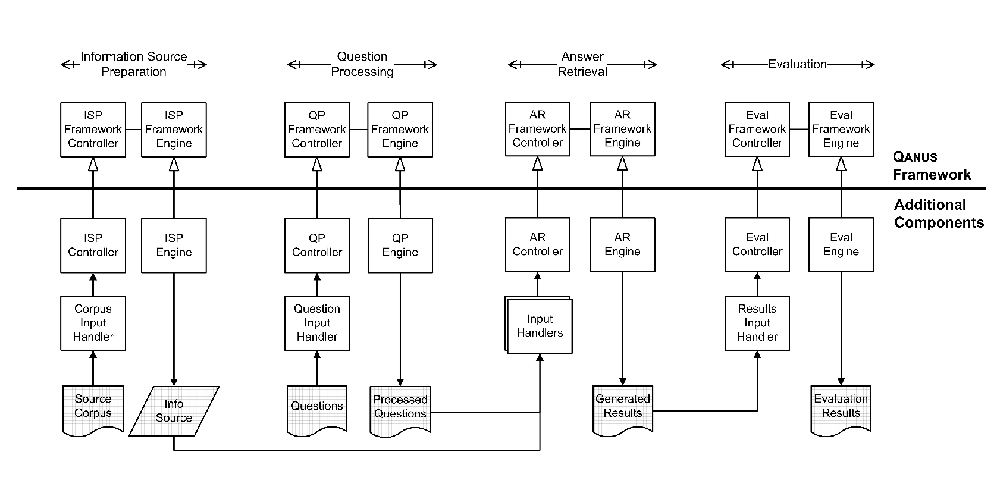
\includegraphics[scale=0.7]{graficos/Quanus}
    \caption{El framework Quanus y la implementación QA-sys}
    \label{fig:Quanus}
  \end{figure}
\end{frame}


\begin{frame}
\frametitle{QA-Sys - Qanus @ Trec 07}
\begin{columns}[T] % align columns
\begin{column}{.48\textwidth}
  \begin{figure}
      \includegraphics[scale=0.5]{graficos/trec-7-accuracy-reduced}
    \caption{Resultados de Trec 07}
    \label{fig:tareas}
  \end{figure}
\end{column}%
\hfill%
\begin{column}{.48\textwidth}

  \begin{block}{TREC 07}
      \begin{itemize}
          \item Monolingue, Inglés. Competencia importante
          \item Una respuesta por pregunta
          \item 200 preguntas en total
          \item Evaluada por humanos
          \item \textit{Precisión}: respuestas exactas sobre respuestas totales
          \item LymbaPA $\rightarrow$ {\color{blue}0.706} (70\%)
          \item QA-Sys $\rightarrow$ {\color{blue}0.119} (12\%)
        \end{itemize}
  \end{block}
\end{column}%
\end{columns}

\end{frame}


\begin{frame}
\frametitle{Baseline: QA-Sys}
  \textbf{1. Preparación de la fuente de información: } Preprocesa XML de Aquaint de manera offline en un índice Lucene. \newline

\textbf{2. Análisis de la pregunta: } \newline Anota la pregunta con POS, NER y QC. \newline

\textbf{3. Generación de respuestas: } Busca la pregunta en el índice, separa los documentos en pasajes y los rankea con métricas heurísticas y luego, dependiendo del tipo de QC, aplica heurísticas basadas en NER, POS y QC sobre los pasajes para extraer una respuesta.\newline

\end{frame}

\begin{frame}
\frametitle{Baseline: ML QA-Sys}
  \begin{itemize}
    \item Soporte multi idioma no simultaneo.
    \begin{itemize}
      \item Soporta varios idiomas, pero de a uno a la vez.
    \end{itemize}
    \item Indice invertido de Wikipedia
    \item Reemplazamos las herramientas NLP por Freeling y sacamos reglas dependiente al idioma.
  \end{itemize}
\end{frame}


\begin{frame}
\frametitle{Pipeline}
  \begin{figure}
      \includegraphics[scale=0.3]{graficos/pipeline}
  \end{figure}
\end{frame}


\begin{frame}
\frametitle{1. Preparación de la base de conocimiento}
  \begin{figure}
      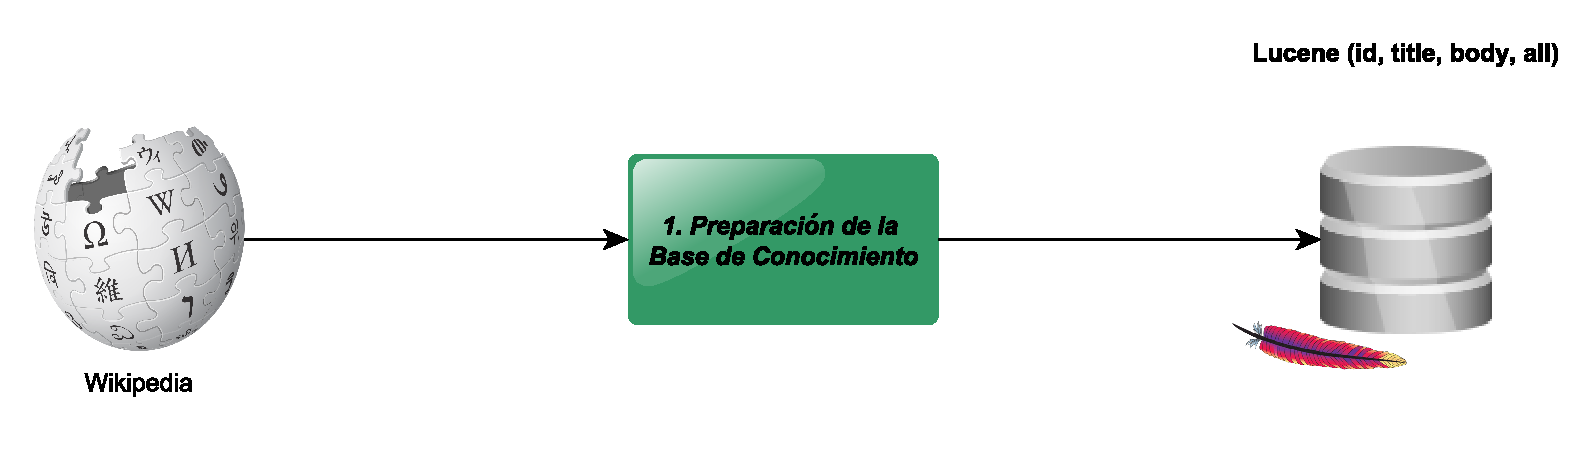
\includegraphics[scale=0.33]{graficos/pipeline-ibp}
  \end{figure}
    \begin{table}
    \centering
    \begin{center}
    \begin{tabular}{| l | l | l | l | l | l| l|}
    Wikipedia & \# Entradas & Nulas & Redirects & Filtradas & \textbf{Válidas} \\ 
    simple-06 & 18273 & 22 &  3452 & 5241 & 9558 \\ 
    simple-13 & 180067 & 8 & 35600 & 41902 & 102557\\
    \textbf{es-06} & \textbf{233750} & 52 & 62805 & 34947 & \textbf{{\color{green}135946}} \\ 
    \textbf{pt-07} & \textbf{498039} & 80 & 210983 & 43390 & \textbf{{\color{green}243586}} \\ 
    \end{tabular}
    \caption{Wikipedias: cantidad de entradas válidas e inválidas}
    \label{table:creacion-indices}
    \end{center}
    \end{table}
\end{frame}


% \begin{frame}
% \frametitle{2. Procesamiento de la pregunta}
%   \begin{figure}
%       \includegraphics[scale=0.3]{graficos/pipeline-qp}
%     \label{fig:Quanus}
%   \end{figure}
% \end{frame}

\begin{frame}
\frametitle{2. Procesamiento de la pregunta}
  \begin{itemize}
    \item NER $\rightarrow$ Freeling
    \item POS $\rightarrow$ Freeling {\color{red} Explicar que es quizas con graficos?}
    \item QC $\rightarrow$ {\color{red}No hay} (tesista?)
    \begin{itemize}
        \item Aprovechando que estaban activas las tareas en-es y en-pt
        \item Hack (truchada)  $\rightarrow$ pasamos QC sobre preguntas en inglés
    \end{itemize}
  \end{itemize}

  \begin{table}
    \centering
    \begin{center}
    \begin{tabular}{| l | l | l | }
    Clase & \# ES  & \# PT \\ 
    HUM &  62 & 53 \\ 
    NUM &  53 & 52\\ 
    ENTY &  34 & 28\\ 
    DESC &  25 & 30\\ 
    LOC &  24 & 36\\ 
    ABBR &  2 & 1\\ 
    Total & 200 & 200 \\
    \end{tabular}
    \caption{Clases de las preguntas para ES y PT, Stanford Classifier (Li \& Roth, Stanford)}
    \label{table:qc-es-pt}
    \end{center}
  \end{table}
\end{frame}


% \begin{frame}
% \frametitle{Pipeline}
%   \begin{figure}
%       \includegraphics[scale=0.3]{graficos/pipeline}
%     \caption{Pipeline}
%     \label{fig:Quanus}
%   \end{figure}
% \end{frame}

\begin{frame}
\frametitle{3. Generación de Respuestas}
  \begin{columns}[T] % align columns
\begin{column}{.38\textwidth}
      \begin{figure}
          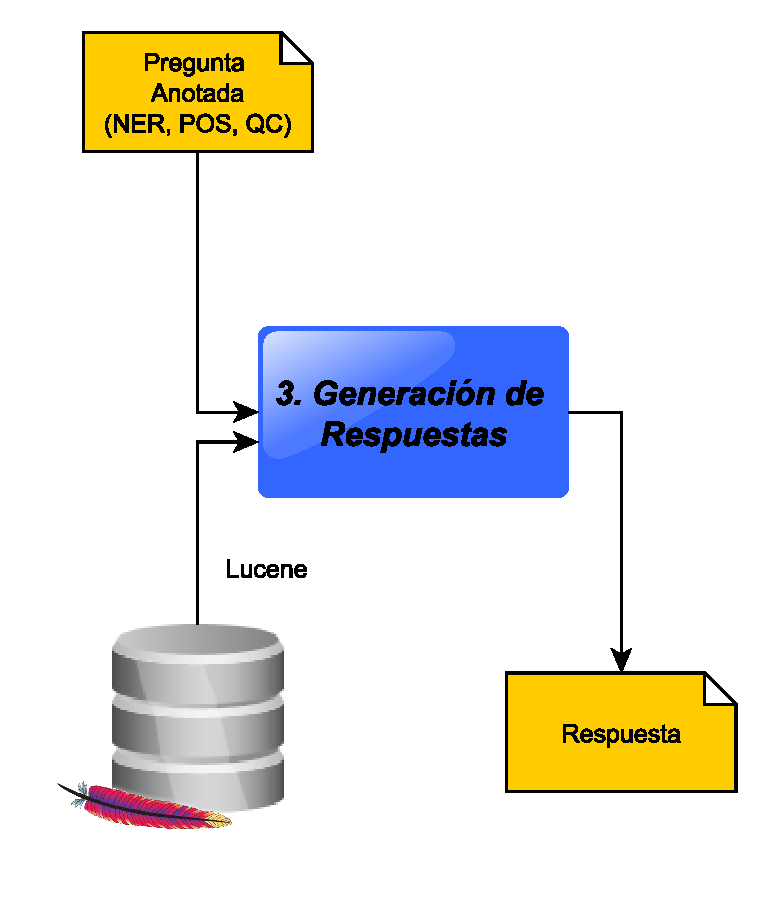
\includegraphics[scale=0.3]{graficos/pipeline-ar}
        %\caption{Módulos y submódulos de un sistema de QA}
        %\label{fig:tareas}
      \end{figure}
\end{column}%
\hfill%
\begin{column}{.58\textwidth}
El algoritmo tiene los siguientes pasos:
  \begin{enumerate}
    \item Filtrado de preguntas
    \item Generación de Queries
    \item Information Retrieval
    \item Extracción y rankeo de oraciones
    \item POS tagging de las mejores oraciones
    \item Heurísticas de AR basadas en el QC
  \end{enumerate}
\end{column}%
\end{columns}
\end{frame}

\begin{frame}
\frametitle{3. Generación de Respuestas (2)}
   \begin{block}{3.1 Filtrado de preguntas}
  \begin{itemize}
      \item Solo factoids (no definition, no list, no nil), solo de wikipedia
      \item Total: 122 es, 104 pt
    \end{itemize}
  \end{block}
  \begin{block}{3.2 Generación de Queries}
  \begin{itemize}
      \item Descartamos caso (\dq{Who (is|was) (the) NN ... NN?} )
      \item 2. Caso baseline
      \begin{itemize}
        \item Espera \sq{target}(TREC) / tópico (Clef) y pregunta. 
        \item Query:
        \begin{itemize}
              \item  Palabras no stop-words de \textit{target} 
              \item  Sustantivos, verbos y adjetivos de la pregunta.
        \end{itemize}
      \end{itemize}
    \end{itemize}
  \end{block}
\end{frame}


\begin{frame}
\frametitle{3. Generación de Respuestas (IR)}
  \begin{block}{3.3, 3.4, 3.5 - IR + Extracción y rankeo de oraciones}
    \begin{itemize}
      \item Documentos divididos en oraciones (no heredan rank)
      \item Peso ponderado por scorers entre 0 y 1:
      \item $rank = 0.9\times covr + 0.05\times freq + 0.05\times prox;$
      \item Primeras $K$ oraciones pos-taggeadas, el resto se desecha
    \end{itemize}
  \end{block}
\end{frame}

\begin{frame}
\frametitle{Scorers: Freq, Cov, Prox}
  \begin{block}{Freq \& Cov: Ocurrencia de la query en la respuesta candidata}
  \begin{itemize}
      \item Frecuencia: tokens de la query que ocurren en la oración sobre tokens de la oración 
      \item Cubrimiento: tokens de que query que ocurren en la oración sobre tokens de la query
  \end{itemize}
  \end{block}
  \begin{block}{Prox: distancia de dos strings en un tercero}
  \begin{itemize}
      \item $s_1=$\dq{Argentina es un país americano} y $s_2=$\dq{independizado en 1810}
      \item $t=$\dq{Argentina es un país americano, originalmente una colonia española, independizado en 1810}
      \item $prox(s_1, s_2, t)= frac{dist(s_1, s_2)}{len(t)} = frac{7}{12} = 0.58 $, 
      \begin{itemize}
          \item $dist(s_1, s_2)=$ cantidad de strings entre \sq{un} y \sq{en} (tokens intermedios de $s_{1,2}$)
          \item $len(t)=$ cantidad de strings del texto
          \item $~$1 denota que los dos string están cercanos uno al otro en el tercer string.
      \end{itemize}
  \end{itemize}
  \end{block}
  \begin{block}{Span: similar a Prox, pero sobre un string y sus tokens}
  \begin{itemize}
  \item $s = \{token_1, token_2, ..., token_n\}$ y $t$ un texto
  \item Sea $r$ la cantidad de tokens de $s$ que aparecen en $t$
  \item Sea $d$ la distancia de los tokens de $s$ más distantes en $t$
  \item Entonces, $\text{Span}=fraq{r}{d}$
  \item Un score cercano a 1 significa que los términos del string buscado están cerca en el string en el que se buscan.
  \item Ejemplo (match es una X):
        ..... X ..... X ..... X ...... \newline
        ......a ...... b ...... c ...... \newline
    $Span$ = \#total de tokens encontrados / $| c - a |$.
  \end{itemize}
  \end{block}
\end{frame}


\begin{frame}
\frametitle{Scorers: Span}
  \begin{block}{Span: similar a Prox, pero sobre un string y sus tokens}
  \begin{itemize}
  \item $s = \{token_1, token_2, ..., token_n\}$ y $t$ un texto
  \item Sea $r$ la cantidad de tokens de $s$ que aparecen en $t$
  \item Sea $d$ la distancia de los tokens de $s$ más distantes en $t$
  \item Entonces, $\text{Span}=fraq{r}{d}$
  \item Un score cercano a 1 significa que los términos del string buscado están cerca en el string en el que se buscan.
  \item Ejemplo (match es una X):
        ..... X ..... X ..... X ...... \newline
        ......a ...... b ...... c ...... \newline
    $Span$ = \#total de tokens encontrados / $| c - a |$.
  \end{itemize}
  \end{block}
\end{frame}


\begin{frame}
  \frametitle{3.6 Heurísticas de AR}
\begin{columns}[T] % align columns
\begin{column}{.48\textwidth}
    \begin{block}{3.6 Heurísticas de AR}
  \begin{itemize}
      \item Basadas en Question Type
      \item Re ranking
      \item Extracción especifica
  \end{itemize}
  \end{block}

\end{column}%
\hfill%
\begin{column}{.48\textwidth}

Casos
  \begin{itemize}
  \item ABBR:exp
  \item ABBR:abb $\rightarrow$ $\emptyset$
  \item HUM:gr y ENTY:cremat
  \item HUM:ind
  \item HUM general
  \item LOC general
  \item NUM:date
  \item NUM:period
  \item NUM:count
  \item NUM general
  \item ENTY general.
\end{itemize}

\end{column}%
\end{columns}
\end{frame}


%%%%%%%%%%%%%%%%%%%%%%%%%%%%%%%%%%%
%%
%%    Casos de Heuristicas de AR
%%
%%%%%%%%%%%%%%%%%%%%%%%%%%%%%%%%%%%


\begin{frame}
  \frametitle{Casos - ABBR:exp}
  \textbf{Caso ABBR:exp - expansión de una abreviación}\newline
  \begin{itemize}
    \item Se extraen las entidades nombradas de tipo \textit{Organización} de la pregunta. 
    \item Se generan regex de expansión de esas abreviaciones. 
    \begin{itemize}
       \item UBA $\rightarrow$ $[U][A-Za-z0-9][B][A-Za-z0-9][A][A-Za-z0-9]$.
    \end{itemize}    
    \item Busca este patrón en las 40 oraciones, devuelve el primer match. \newline
  \end{itemize}
\end{frame}


\begin{frame}
\frametitle{Casos - HUM:gr y ENTY:cremat}
\textbf{Caso HUM:gr y ENTY:cremat - grupos humanos (compañías, organizaciones) y objetos humanos (libros, inventos, discos, etc)} \newline
  \begin{itemize}
    \item Respuestas candidatas $\rightarrow$ extraer nombres propios (proper nouns, NNPs) de todas las oraciones rankeadas .
      \begin{itemize}
        \item Nombres propios consecutivos se agrupan (Tiger Woods)/NNP 
    \end{itemize}
    \item \st{Filtro candidatas que contengan palabras en diccionario.} \footnotemark
    \item Re ranking de las candidatas según scores: 
    \begin{itemize}
        \item \tiny{$Total = 0.55 * Coverage + 0.2 * Sentence + 0.1 * Proximity + 0.15 * RepeatedTerm$}
        \item \tiny{$Coverage$: cubrimiento del target en la oración de soporte}
        \item \tiny{$Proximity$: distancia entre el target y la respuesta candidata en la oración}
        \item \tiny{$Sentence$: posición de la oración en las 40 seleccionadas}
        \item \tiny{$RepeatedTerm$: penalización. negativa. si la respuesta candidata tiene tokens en común con el target}
    \end{itemize}
  \end{itemize}

  \footnotetext[1]{\tiny{En concreto: \{Monday, Tuesday, Wednesday, Thursday, Friday, Saturday, Sunday\}, \{January, February, March, April, May, June, July, August, September, October, November, December\}, y \{us, uk, france, england, cuba, japan, u.s, america\}.}}
\end{frame}

\begin{frame}
  \frametitle{Casos - HUM:ind - individuo humano}
  \textbf{Caso HUM:ind - individuo humano}
  %\ChangeItemFont{\footnotesize}{\footnotesize}{\footnotesize}
  \begin{itemize}
    \item Respuestas candidatas = Extraer NER tipo \textit{PERSON} de las oraciones.
    \item Score: $0.5 \times CoverageTarget+ 0.25 \times CoverageSubject + 0.35 \times Sentence +
               0.25 \times Proximity  + 0.1 \times RepeatedTerm + 0.5 \times IsPronoun$
    \begin{itemize}
      \item \tiny{CoverageTarget: cuántos tokens del target aparecen en la oración fuente de la respuesta candidata}
      \item \tiny{CoverageSubject: cuántos tokens del subject aparecen en la oración fuente de la respuesta candidata (si se pudo encontrar un subject, cero si no - en nuestra adaptación es siempre cero)}
      \item \tiny{Sentence: derivado de la posición de la oración en el ranking}
      \item \tiny{Proximity: cuán cerca están la query utilizada como input del módulo de information retrieval (sin stop-words) y la respuesta candidata en el contexto de la oración de la que se extrajo la respuesta candidata.}
      \item \tiny{RepeatedTerm: penalización (negativo). Coverage entre el target y la respuesta candidata}
      \item \tiny{IsPronoun: Penaliza si la respuesta candidata contiene pronombres. En concreto, verifica si algún token pertenece a la lista \{it, we, he, she, they, our, their\}.}
    \end{itemize}
  \end{itemize}

\end{frame}


\begin{frame}
\frametitle{Casos - otros casos}

\textbf{HUM general y ENTY general:} - otros temas humanos y otros objetos - Primer nombre propio de la oración mejor rankeada y se utiliza eso como respuesta. \newline

\textbf{LOC general:} - preguntas que refieren a lugares - Se extraen todas las entidades nombradas de tipo \sq{LOCATION} de las oraciones rankeadas y se las evalúa según un score ponderado \newline
%de cubrimiento, posición en el ranking de oraciones, proximidad y penalización por repeticiones.

% $TotalScore = (0.6 * CoverageScore) + (0.1 * SentenceScore) + (0.2 * ProximityScore)  + (0.5 * SanityScore) + (0.3 * RepeatedTermScore)$ \newline

% Donde los scores representan lo siguiente:
% \begin{itemize}
%   \item CoverageScore: cuántos tokens del \sq{target} aparecen en la oración fuente de la respuesta candidata
%   \item SentenceScore: puntaje derivado de la posición de la oración-fuente en el ranking de oraciones
%   \item ProximityScore: cuán cerca están la query utilizada como input del módulo de information retrieval (sin stop-words) y la respuesta candidata en el contexto de la oración de la que se extrajo la respuesta candidata.
%   \item RepeatedTermScore: penalización (negativo). Coverage entre el \sq{target} y la respuesta candidata.
%   \item SanityScore: es un placeholder para implementar código comentado. En el código que encontramos, vale 1 (constante).
% \end{itemize}
\textbf{Casos NUM} - fechas, períodos, cuentas y números en general -
\begin{itemize}
\item La primer fecha encontrada según rank de pasajes (NUM:Date)
\item El primer número encontrado según pasajes (NUM:Count)
\item El primer numérico (número o fecha) para los otros casos NUM
\end{itemize}


\end{frame}


\begin{frame}
\frametitle{Modificaciones}
  \begin{itemize}
    \item Inferencia del tópico del grupo de preguntas
    \item Generación de queries
    \item Generación de respuestas
  \end{itemize}
\end{frame}

\begin{frame}
\frametitle{Inferencia del tópico del grupo de preguntas}
  \begin{itemize}
    \item Grupos de 1 a 4 preguntas con tema
    \item Ejemplos: Colegio de Harry Potter, Pez Espada, Revolución de Terciopelo
    \item Condiciones del tema
    \begin{itemize}
      \item Nombrado en primer pregunta/respuesta
      \item Las siguientes preguntas pueden contener correferencias a este tópico
    \end{itemize}
    \item Incorporado al sistema como "Target"
    \item Probamos diferentes valores:
    \begin{enumerate}
      \item Test (el del test set)
      \item NERs + Numeros + Fechas
      \item Sustantivos
      \item 2 y 3
    \end{enumerate}
    \item 2, 3 y 4 basados solo en la 1er pregunta del cluster.
  \end{itemize}
\end{frame}

\begin{frame}
\frametitle{Generación de queries}
  \begin{enumerate}
    \item Baseline / Qanus: 
    \begin{itemize}
      \item Tokens no repetidos ni stopwords de target (tópico)
      \item Sustantivos, verbos y adjetivos de la pregunta completa
      \item {\color{blue} + números + fechas}
    \end{itemize}
    \item Baseline \dq{mejorado}: \textit{(TITLE: target)$^n$ OR \textbf{query baseline}},  $n=5$
    \item Lasso: como describimos en Estado de Arte
      \begin{enumerate}
        \item Palabras no stop words entre comillas
        \item NERs
        \item Construcciones nominales con sus adjetivos
        \item Demás construcciones nominales
        \item Sustantivos con sus adjetivos
        \item Demás sustantivos
        \item Verbos
        \item \st{El focus de la pregunta}
        \end{enumerate}
  \end{enumerate}


\end{frame}

\begin{frame}
\frametitle{Generación de respuestas}
%\ChangeItemFont{\scriptsize}{\scriptsize}{\scriptsize}
  \begin{itemize}
    \item Scorers nuevos para rankear los pasajes
    \item No tocamos las heurísticas
    \item Scorers:
    \begin{itemize}
      \item Length : Prioriza oraciones cortas pero no demasiado cortas.
      \item QVerb: Presencia de verbos de la pregunta en la oración.
      \item QNoun: Presencia de sustantivos.
      \item QNER: Presencia de NERs.
      \end{itemize}
      \item Tres métodos de rankeo de pasajes: \newline
        $pscore_{bl} = 0.9 \times Coverage + 0.05 \times Freq + 0.05 \times Prox;$ \newline
        $pscore_2 = 0.4 \times pscore_{bl} + 0.2 \times QNER +  0.15 \times QVerb + 0.25 \times QNoun$ \newline
        $pscore_3 =  0.4 \times pscore_{bl} + 0.15 \times Length + 0.1 \times QNER + 0.1 \times QVerb + 0.1 \times QNoun$
  \end{itemize}
\end{frame}



%%%%%%%%%%%%%%%%%%%%%%%%%%%%%%%%%%%
%%
%%      Experimentación
%%
%%%%%%%%%%%%%%%%%%%%%%%%%%%%%%%%%%%


\subsubsection*{Experimientación}
\begin{frame}
\frametitle{Experimentos}
Corridas
\begin{itemize}
  \item Idioma: español, portugués (2 opciones)
  \item Documentos retornados por Lucene: 50, 100, 200 (3 opciones)
  \item Pasajes extraídos de los documentos: 20, 40, 70 (3 opciones)
  \item Generación de Queries: baseline (1), improved baseline (2), lasso (3) (3 opciones)
  \item Inferencia de Temas: Test (1), NERs (2), sustantivos (3), híbrido (4) (4 opciones)
  \item Ranking de Pasajes: baseline (1), 2, 3 (3 opciones)
\end{itemize}

Evaluación de resultados
\begin{itemize}
  \item Cantidad de respuestas dadas por el sistema: 1, 5, 10, 25 (4 opciones)
  \item Forma de evaluación automática: exacto, cubrimiento del 100\%, 75\% y 50\%, 15\%  y 1\% (6 opciones)
\end{itemize}
\end{frame}

\begin{frame}
\frametitle{Corrida 1: instanciación de cantidades}

\begin{itemize}
  \item Idioma: Español
  \item \textbf{{\color{blue}Documentos retornados por Lucene: 50, 100, 200}}
  \item \textbf{{\color{blue} Pasajes extraídos de los documentos: 20, 40, 70}}
  \item Generación de Queries: Baseline (1)
  \item Inferencia de Temas: NERs propio (2)
  \item Ranking de Pasajes: Baseline (1)
\end{itemize}

\end{frame}

\begin{frame}
\frametitle{Corrida 1: resultados}

\begin{table}
\centering
\begin{center}
\begin{tabular}{|l | l | l | l | l | l | l |}

Medida & Exacto & Covr 1 & Covr .75 & Covr .5 & Covr .15 & Covr .01 \\ 
$MRR_{1}$ & 7.69 & 7.69 & 8.46 & 10.00 & 10.00 & 10.00  \\ 
$MRR_{5}$ & 8.87 & 9.18 & 9.95 & \textbf{12.51} & \textbf{13.47} & \textbf{13.54}  \\ 
$MRR_{10}$ & \textbf{9.37} & \textbf{9.44} & \textbf{10.21} & \textbf{12.77} & \textbf{14.25} & \textbf{14.31}  \\ 
$MRR_{25}$ & \textbf{9.56} & \textbf{9.63} & \textbf{10.40} & \textbf{13.07} & \textbf{14.58} & \textbf{14.65}  \\ 
\end{tabular}

\medskip
\medskip

\begin{tabular}{|l | l | l | l | l | l | l |}
Medida & Exacto & Covr 1 & Covr .75 & Covr .5 & Covr .15 & Covr .01 \\ 
$MRR_{1}$ & \textbf{7.75} & \textbf{7.75} & \textbf{8.53} & \textbf{10.08} & \textbf{10.08} & \textbf{10.08}  \\ 
$MRR_{5}$ & \textbf{8.94} & \textbf{9.25} & \textbf{10.03} & 12.42 & 13.39 & 13.45  \\ 
$MRR_{10}$ & 9.31 & 9.38 & 10.16 & 12.55 & 14.03 & 14.10  \\ 
$MRR_{25}$ & 9.54 & 9.61 & 10.39 & 12.89 & 14.41 & 14.48  \\ 
\end{tabular}
\caption{Corrida 1: con 50 documentos de Lucene y 20, 40 pasajes}
\end{center}
\end{table}

Observaciones y conclusiones
\begin{itemize}
  \item 9 ejecuciones en total
  \item Más documentos de Lucene, peor en todas las permutaciones
  \item Muchos pasajes (70) también es malo en general
  \item 20 y 40 se comportan raro. $\rightarrow$ 40 es mejor para evaluaciones más exactas
  \item Fijamos 50 y 40 para el resto de las corridas
\end{itemize}

\end{frame}


\begin{frame}
\frametitle{Corrida 2.1: Generación de Queries}

\begin{itemize}
  \item Idioma: Español
  \item Documentos retornados por Lucene: \textbf{50}
  \item Pasajes extraídos de los documentos: \textbf{40}
  \item \textbf{{\color{blue}Generación de Queries: Baseline, Baseline mejorado, Lasso}}
  \item Inferencia de Temas: NERs propio (2)
  \item Ranking de Pasajes: Baseline (1)
\end{itemize}

\end{frame}

\begin{frame}
\frametitle{Corrida 2.1: Resultados}


\begin{table}
\centering
\begin{center}
\begin{tabular}{|l | l | l | l | l | l | l |}

& \multicolumn{2}{|c|}{Baseline} & \multicolumn{2}{|c|}{Baseline mejorado} & \multicolumn{2}{|c|}{Lasso}\\ 
Medida & Exacto & Covr 1 & Exacto & Covr 1 & Exacto & Covr 1 \\ 

\textbf{$MRR_{1}$} & \textbf{7.75} & \textbf{7.75} &  \textbf{3.91} & \textbf{3.91} & \textbf{{\color{green}7.81}} & \textbf{{\color{green}7.81}} \\ 
$MRR_{5}$ & \textbf{8.94} & \textbf{9.25} &  \textbf{5.36} & \textbf{5.91} & \textbf{9.27} & \textbf{9.58}   \\ 
$MRR_{10}$ & 9.31 & 9.38 &  5.96 & 6.43 & 9.64 & 9.71   \\ 
$MRR_{25}$ & 9.54 & 9.61 &  5.96 & 6.43 & 9.94 & 10.01  \\ 
\end{tabular}

\caption{Corrida 2.1: Generación de Queries}
\end{center}
\end{table}

Observaciones y Conclusiones
\begin{itemize}
  \item Método lasso ligeramente superior a baseline
  \item Baseline \dq{mejorado} rezagado siempre
\end{itemize}

\end{frame}


\begin{frame}
\frametitle{Corrida 2.2: Inferencia de Temas}

\begin{itemize}
  \item Idioma: Español
  \item Documentos retornados por Lucene: 50
  \item Pasajes extraídos de los documentos: 40
  \item Generación de Queries: \textbf{Baseline}
  \item \textbf{{\color{blue}Inferencia de Temas: Test (1), NERs (2), sustantivos (3), híbrido (4)}}
  \item Ranking de Pasajes: Baseline (1)
\end{itemize}

\end{frame}

\begin{frame}
\frametitle{Corrida 2.2: Resultados}

\begin{table}
\centering
\begin{center}
\begin{tabular}{|l | l | l | l | l |}

& \multicolumn{2}{|c|}{1) Test} & \multicolumn{2}{|c|}{2) NERs}  \\ 
Medida & Exacto & Covr 1 & Exacto & Covr 1 \\ 
$MRR_{1}$ & 6.15 & 6.15 & \textbf{{\color{green}7.75}} & \textbf{{\color{green}7.75}} \\ 
$MRR_{5}$ & 7.87 & 8.41 & \textbf{{\color{green}8.94}} & \textbf{{\color{green}9.25}}  \\ 
$MRR_{10}$ & 8.08 & 8.49 & 9.31 & 9.38  \\ 
$MRR_{25}$ & 8.29 & 8.72 & 9.54 & 9.61  \\ 
\end{tabular}

\medskip

\begin{tabular}{|l | l | l | l | l |}

& \multicolumn{2}{|c|}{3) Sustantivos} & \multicolumn{2}{|c|}{4) 2+3} \\ 
Medida & Exacto & Covr 1 & Exacto & Covr 1 \\ 
$MRR_{1}$ & 3.85 & 3.85 & 5.47 & 5.47 \\ 
$MRR_{5}$ & 4.19 & 4.19 & 7.12 & 7.43 \\ 
$MRR_{10}$ & 4.19 & 4.30 & 7.36 & 7.43 \\ 
$MRR_{25}$ & 4.47 & 4.58 & 7.64 & 7.71 \\ 
\end{tabular}
\caption{Corrida 2.2: Métodos 1, 2, 3 y 4 respectivamente}
\end{center}
\end{table}

Conclusiones:
\begin{itemize}
 \item El método utilizado (NERs + números de la primer pregunta como target) es el más efectivo en todos los casos.
 \item {\color{red}Esto es raro en relación al método 1}
\end{itemize}


\end{frame}


\begin{frame}
\frametitle{Corrida 2.3: Ranking de Pasajes}

\begin{itemize}
  \item Idioma: Español
  \item Documentos retornados por Lucene: 50
  \item Pasajes extraídos de los documentos: 40
  \item Generación de Queries: Baseline
  \item Inferencia de Temas: \textbf{NERs (2)}
  \item \textbf{{\color{blue}Ranking de Pasajes:  Baseline (1), $pscore_2$, $pscore_3$}}
\end{itemize}
\end{frame}

\begin{frame}
\frametitle{Corrida 2.3: Resultados}
\begin{table}
\centering
\begin{center}

\begin{tabular}{|l | l | l | l | l | l | l |}

& \multicolumn{2}{|c|}{$PassageScore_{bl}$} & \multicolumn{2}{|c|}{$PassageScore_2$} & \multicolumn{2}{|c|}{$PassageScore_3$}\\ 
Medida & Exacto & Covr 1 & Exacto & Covr 1 & Exacto & Covr 1 \\ 
$MRR_{1}$ & 7.75 & 7.75 & 3.10 & 3.10 & 5.38 & 5.38  \\ 
$MRR_{5}$ & 8.94 & 9.25 & 5.06 & 5.22 &  6.69 & 6.85  \\ 
$MRR_{10}$ & 9.31 & 9.38 & 5.35 & 5.50 &  7.15 & 7.31  \\ 
$MRR_{25}$ & 9.54 & 9.61 & 5.39 & 5.55 &  7.19 & 7.35  \\ 
\end{tabular}
\caption{Corrida 2.3: Fórmulas 1, 2 y 3 respectivamente}
\end{center}
\end{table}

Observaciones y conclusiones
\begin{itemize}
  \item Todo mal
  \item diff $pscore_2$ y $pscore_3$ $\rightarrow$ $LengthScore$ 
  \begin{itemize}
    \item Único agregado sustantivo a $pscore_3$
    \item Aplicarlo al baseline
  \end{itemize}
  \item Nuevas corridas con LenghtScore: 90/10 80/20 y 70/30
  \item La fórmula del score es la siguiente:
    \begin{equation*}
        LengthScore = \begin{cases}
                   1.0     & 4 <   \#tokens < 100\\
                   0.5     & 100 \leq \#tokens < 200 \\
                   0.0     & \text{En cualquier otro caso}\\
               \end{cases}
    \end{equation*}
  \end{itemize}

\end{frame}

\begin{frame}
\frametitle{Corrida 2.3: Resultados 2}

\begin{table}
\centering
\begin{center}
\begin{tabular}{|l | l | l | l | l | l | l |}

& \multicolumn{2}{|c|}{0.9 + 0.1} &
  \multicolumn{2}{|c|}{0.8 + 0.2} &
  \multicolumn{2}{|c|}{0.7 + 0.3} \\ 
Medida & Exacto & Covr 1 & Exacto & Covr 1 & Exacto & Covr 1 \\ 
$MRR_{1}$ & 7.81 & 7.81 & \textbf{10.08} & \textbf{10.08} & 10.00 & 10.00  \\ 
$MRR_{5}$ & 9.47 & 9.78 & 11.68 & 11.99 & 11.94 & 12.50  \\ 
$MRR_{10}$ & 9.71 & 9.78 & 11.92 & 11.99 & 12.35 & 12.67  \\ 
$MRR_{25}$ & 10.01 & 10.08 & 12.27 & 12.34 & 12.58 & 12.91  \\ 
\end{tabular}
\caption{Corrida 2.3: Combinación ponderada de métodos 1 y 3}
\end{center}
\end{table}


Observaciones y conclusiones
\begin{itemize}
  \item El score funciona como filtro de pasajes mal formados o bien formados pero largos. En ambos casos, NLP pierde eficacia.
  \item Mejor resultado cuando más ponderacion salvo $MRR_1$ que se redujo en la tercer corrida. 
  \begin{itemize}
    \item Dado que esta métrica es la preferida, decidimos quedarnos con esta fórmula (8/2 y no 7/3)
    \end{itemize}
  \item Mejoras fáciles acá.
  \end{itemize}

\end{frame}



\begin{frame}
\frametitle{Corrida 3: Combinación de Óptimos}

\medskip

Datos de la corrida 3.1, para español:
\begin{itemize}
  \item Idioma: Español
  \item Documentos retornados por Lucene: 50
  \item Pasajes extraídos de los documentos: 40
  \item Generación de Queries: Baseline
  \item Inferencia de Temas: NERs (2)
  \item Ranking de Pasajes: $PassageScore_{bl} \times 0.8 + LengthScore \times 0.2$
\end{itemize}

\medskip
Datos de la corrida 3.2, para portugués:
\begin{itemize}
  \item Idioma: {\color{blue}Portugués}
  \item Documentos retornados por Lucene: 50
  \item Pasajes extraídos de los documentos: 40
  \item Generación de Queries: Baseline
  \item Inferencia de Temas: NERs (2)
  \item Ranking de Pasajes: $PassageScore_{bl} \times 0.8 + LengthScore \times 0.2$
\end{itemize}

\end{frame}

\begin{frame}
\frametitle{Corrida 3: Resultados}


\begin{table}
\centering
\begin{center}
\begin{tabular}{|l | l | l | l | l | l | l |}

Medida & Exacto & Covr 1 & Covr .75 & Covr .5 & Covr .15 & Covr .01 \\ 
$MRR_{1}$ & {\color{green}\textbf{10.65}} & 10.65 & 10.77 & 12.31 & 13.08 & 13.08  \\ 
$MRR_{5}$ & {\color{green}\textbf{12.00}} & 12.31 & 13.46 & 16.18 & 16.95 & 17.01  \\ 
$MRR_{10}$ & 12.24 & 12.31 & 13.46 & 16.26 & 17.44 & 17.50  \\ 
$MRR_{25}$ & 12.55 & 12.62 & 13.78 & 16.72 & 18.00 & 18.06  \\ 
\end{tabular}
\medskip
\caption{Corrida 3.1: Combinación de óptimos para español}
\label{table:optimos}
\end{center}
\end{table}

\begin{table}
\centering
\begin{center}
\begin{tabular}{|l | l | l | l | l | l | l |}

Medida & Exacto & Covr 1 & Covr .75 & Covr .5 & Covr .15 & Covr .01 \\ 
$MRR_{1}$ & {\color{green}\textbf{1.92}} & 2.88 & 2.88 & 3.85 & 3.85 & 3.85  \\ 
$MRR_{5}$ & {\color{green}\textbf{3.16}} & 5.03 & 5.03 & 6.91 & 7.15 & 7.15  \\ 
$MRR_{10}$ & 3.45 & 5.33 & 5.33 & 7.33 & 7.71 & 7.86  \\ 
$MRR_{25}$ & 4.08 & 6.00 & 6.00 & 8.21 & 8.84 & 8.94  \\ 
\end{tabular}
\caption{Corrida 3.2: Combinación de óptimos sobre portugués}
\label{table:2_3_2_40_getExactMRRWikiFactoid_getCovrMRRWikiFactoid}
\end{center}
\end{table}

\end{frame}


\begin{frame}
\frametitle{Resultados de competidores de Clef '07}

\begin{columns}[T] % align columns
\begin{column}{.48\textwidth}
  \begin{figure}
      \includegraphics[scale=0.4]{graficos/resultados-espaniol-resumen}
    \caption{Competidores español}
  \end{figure}
\end{column}%
\hfill%
\begin{column}{.48\textwidth}

  \begin{figure}
      \includegraphics[scale=0.4]{graficos/resultados-portugues}
    \caption{Competidores portugués}
  \end{figure}
\end{column}%
\end{columns}

\end{frame}


\begin{frame}
\frametitle{Corrida 3: observaciones y conclusiones}

\begin{itemize}
  \item Métodos que mejores resultados dieron para español
  \item Quizás, mal extrapolados a portugués
  \item Español peor que en 2.3 para muchas métricas
  \item Portugués: baja performance
  \begin{itemize}
    \item Apenas un 3.16\% considerando la métrica $MRR_5$. 
    \item Las herramientas para portugués no son tan maduras como las herramientas para español; 
    \item Todo el desarrollo y el análisis estuvo basado en español
    \item Solo POC de soporte para otros idiomas
  \end{itemize}
  \item Español: 10.65\% exacto con una sola respuesta! 
  \item No es el peor
\end{itemize}
\begin{itemize}
  \item $10.65\% = \frac{13}{122}$
  \item $1.92\% = \frac{2}{104}$
\end{itemize}
\end{frame}




\begin{frame}
\frametitle{Corrida 3: Respuestas ES}
\fontsize{7.5pt}{7.2}\selectfont
\begin{table}
\centering
\begin{center}
\begin{tabular}{|p {6cm} | l |}

Q & A\\ 
¿De dónde es típica la ensaimada? & Mallorca \\
¿De cuántos bits era este procesador? & 8 bits \\
¿En qué fecha El Corte Inglés compró Galerías Preciados? &  24 de noviembre de 1995\\
¿Qué empresa preside Steve Jobs? &  Apple Computer \\
¿Dé qué organización es comisionado David Stern? &  NBA\\
¿Qué animales tiran del carro de Cibeles? & leones\\
¿Cuántos Premios Goya ganó \dq{Torrente: El brazo tonto de la ley}? & dos\\
¿Quién fue la primera mujer que viajó al espacio? & Valentina Vladimírovna Tereshkova\\
¿A cuántos kilómetros de Huesca está el Castillo de Loarre? &   35 kilómetros\\
¿Cuál es el nombre del presidente de Burundi que murió en 1994? &  Cyprien Ntaryamira\\
¿Qué día se promulgó la constitución española de 1812?  & 19 de marzo\\
¿Qué dibujó Leonardo Da Vinci en 1492? & Hombre de Vitruvio\\
¿Qué programa de televisión presentó Takeshi Kitano de 1986 a 1989? &   Humor Amarillo\\
\end{tabular}
\caption{Respuestas español}
\end{center}
\end{table}
\end{frame}

\begin{frame}
\frametitle{Corrida 3: Respuestas PT}

\begin{table}
\centering
\begin{center}
\begin{tabular}{| p {7cm} | l |}
Q & A\\ 
De que estado foi governador Adhemar de Barros? & São Paulo\\
Quando foi fundado o Nacional da Madeira? & 8 de Dezembro de 1910\\
\end{tabular}
\caption{Respuestas portugués}
\end{center}
\end{table}


\end{frame}




\subsubsection*{Limitaciones, trabajo futuro, conclusiones}

\begin{frame}
\frametitle{Limitaciones y trabajo futuro}
\begin{itemize}
  \item Módulo multilingüe de Question Classification.
  \item Inferencia del tópico a partir del primer par de pregunta-respuesta.
  \item Generación del \textit{focus}. Tema aparte.
  \item Preguntas de tipo definition y list, booleanas, cláusulas temporales.
  \item Mejorar las heurísticas
\end{itemize}

\end{frame}


\begin{frame}
\frametitle{Conclusiones: Dominio abierto}
  \begin{itemize}
    \item Sistema de question answering de dominio abierto con soporte para diferentes idiomas
    \item Qanus, Qa-sys monolingüe + Freeling + Lasso + Scorers
    \item CLEF'07 español y portugués + solo wikipedia + solo factoid + diferentes configuraciones
    \item CLEF'07: la mejor precisión general bajó del 49\% al 41.75\% para tareas multi-lingües, mientras que, más significativamente, bajó de 68\% a 54\% en tareas monolingües
    \item nos restringimos a una subsección sencilla (eliminando preguntas de tipo DEFINITION y LIST), por lo que no es del todo válido comparar esta performance con la nuestra.
    \item Qasys, el sistema baseline que adaptamos para soportar diferentes idiomas, sabemos que en la TREC 07 (en inglés), competencia en la que Qasys participó, el mejor sistema, LumbaPA07, obtuvo una exactitud de 70,06\%, mientas que el décimo (Quanta) obtuvo 20,6\% y Qasys logró un 11,9\%.
\item Nuestro sistema adaptado al español, con todas las mejoras en su óptimo, logra un nada despreciable 10,08 para $MRR_1$ y un 12,00 para $MRR_5$.
  \end{itemize}

\end{frame}

\begin{frame}
\frametitle{Conclusiones 2}

Sobre modelo de dominio abierto:
  \begin{itemize}
 \item Limitación de las mejoras a zonas acotadas y sin enfoques sistémicos. 
 \item Una mejora argumentada y con cierta presencia en la literatura del área fue el mecanismo de generación de queries que llamamos Lasso (por el sistema en el que fue implementado por primera vez) y nosotros lo incorporamos aquí, 
\begin{itemize}
    \item  mejoras mínimas en la performance, de 7.75 a 7.81 en $MRR_1$ exacto (+0.26), de 8.94 a 9.27 en $MRR_5$ exacto (+0.31). 
  \end{itemize}
  \item Falta de "doctrina" en la generación de respuestas. Oportunidad! Linea muerta? 
\item Módulo de \textit{focus} open source en inglés. Problema acotado, bien definido. Herramienta útil
  \end{itemize}
\end{frame}



\section{Cierre}
  \subsection*{Resumen y conclusiones generales}
    \begin{frame}
    \frametitle{Resumen y conclusiones}
      \begin{itemize}
        \item {\color{red} FILL ME}
      \end{itemize}
    \end{frame}

  \subsection*{Preguntas}
  \begin{frame}
    \frametitle{¿Preguntas?}
      \begin{figure}
        \includegraphics[width=9cm,height=6cm]{graficos/qmark2.pdf}
      \end{figure}
    \end{frame}


% \begin{frame}
% \frametitle{Baseline}
%   \begin{itemize}
%     \item {\color{red} FILL ME}
%   \end{itemize}
% \end{frame}


% \begin{frame}
%     \frametitle{Título de la primera diapositiva}
% \begin{columns}
%  \begin{column}{0.55\textwidth}
% \begin{block}{Resultados}
%     \begin{itemize}[<+->]
%       \item  Primer item
%       \item  Segundo item
%       \item  Tercer item
%     \end{itemize}
%     \begin{enumerate}[<+-| alert@+>]
%       \item  Primer item
%       \item  Segundo item
%       \item  Tercer item
%     \end{enumerate}
% \end{block}
%  \end{column} \ \
% % \begin{column}{0.40\textwidth}
%       %\only<4>{\includegraphics[width=0.8\textwidth]{knuth.jpg}}
%       %\only<5>{\includegraphics[width=0.9\textwidth]{forges.jpg}}
%    %   \only<6>{\includegraphics[width=0.9\textwidth]{kill-bill-2.jpg}}
% % \end{column}
% \end{columns}
% \end{frame}



\end{document}

% \usetheme{default}
% \usetheme{JuanLesPins}
% \usetheme{Goettingen}
% \usetheme{Szeged}
% \usetheme{Warsaw}

% \usecolortheme{crane}

% \usefonttheme{serif}
% \usefonttheme{structuresmallcapsserif}
